\begin{figure}[!h]
\centering
\resizebox{\textwidth}{!}{%
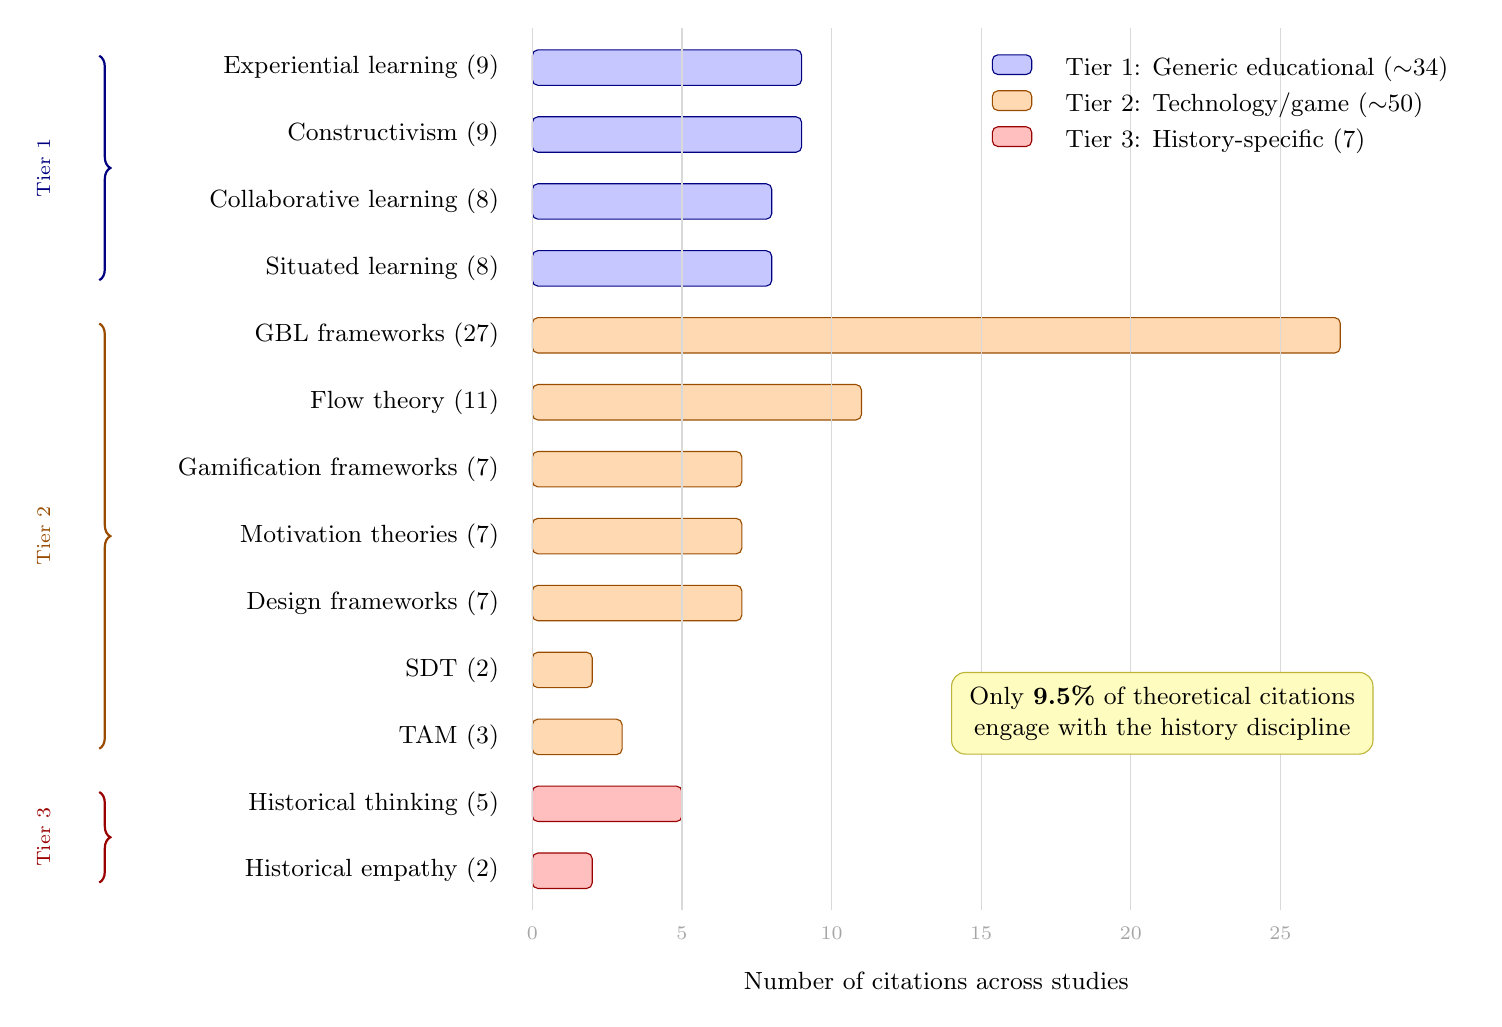
\begin{tikzpicture}

% Bar dimensions
\def\barheight{0.45}
\def\yscale{0.85}
\def\xscale{0.38}

% Tier labels (right-aligned y-axis labels)
\foreach \y/\label in {
    0/{Historical empathy (2)},
    1/{Historical thinking (5)},
    2/{TAM (3)},
    3/{SDT (2)},
    4/{Design frameworks (7)},
    5/{Motivation theories (7)},
    6/{Gamification frameworks (7)},
    7/{Flow theory (11)},
    8/{GBL frameworks (27)},
    9/{Situated learning (8)},
    10/{Collaborative learning (8)},
    11/{Constructivism (9)},
    12/{Experiential learning (9)}
} {
    \node[font=\small, anchor=east] at (-0.3, \y*\yscale) {\label};
}

% Tier 3 — History-discipline-specific (red)
\fill[red!25, draw=red!60!black, rounded corners=2pt] (0, 0*\yscale-\barheight/2) rectangle (2*\xscale, 0*\yscale+\barheight/2);
\fill[red!25, draw=red!60!black, rounded corners=2pt] (0, 1*\yscale-\barheight/2) rectangle (5*\xscale, 1*\yscale+\barheight/2);

% Tier 2 — Technology/game-specific (orange)
\fill[orange!30, draw=orange!60!black, rounded corners=2pt] (0, 2*\yscale-\barheight/2) rectangle (3*\xscale, 2*\yscale+\barheight/2);
\fill[orange!30, draw=orange!60!black, rounded corners=2pt] (0, 3*\yscale-\barheight/2) rectangle (2*\xscale, 3*\yscale+\barheight/2);
\fill[orange!30, draw=orange!60!black, rounded corners=2pt] (0, 4*\yscale-\barheight/2) rectangle (7*\xscale, 4*\yscale+\barheight/2);
\fill[orange!30, draw=orange!60!black, rounded corners=2pt] (0, 5*\yscale-\barheight/2) rectangle (7*\xscale, 5*\yscale+\barheight/2);
\fill[orange!30, draw=orange!60!black, rounded corners=2pt] (0, 6*\yscale-\barheight/2) rectangle (7*\xscale, 6*\yscale+\barheight/2);
\fill[orange!30, draw=orange!60!black, rounded corners=2pt] (0, 7*\yscale-\barheight/2) rectangle (11*\xscale, 7*\yscale+\barheight/2);
\fill[orange!30, draw=orange!60!black, rounded corners=2pt] (0, 8*\yscale-\barheight/2) rectangle (27*\xscale, 8*\yscale+\barheight/2);

% Tier 1 — Generic educational (blue)
\fill[blue!22, draw=blue!50!black, rounded corners=2pt] (0, 9*\yscale-\barheight/2) rectangle (8*\xscale, 9*\yscale+\barheight/2);
\fill[blue!22, draw=blue!50!black, rounded corners=2pt] (0, 10*\yscale-\barheight/2) rectangle (8*\xscale, 10*\yscale+\barheight/2);
\fill[blue!22, draw=blue!50!black, rounded corners=2pt] (0, 11*\yscale-\barheight/2) rectangle (9*\xscale, 11*\yscale+\barheight/2);
\fill[blue!22, draw=blue!50!black, rounded corners=2pt] (0, 12*\yscale-\barheight/2) rectangle (9*\xscale, 12*\yscale+\barheight/2);

% X-axis
\draw[gray!50] (0, -0.5) -- (0, 12*\yscale+0.5);
\foreach \x in {0, 5, 10, 15, 20, 25} {
    \draw[gray!30] (\x*\xscale, -0.5) -- (\x*\xscale, 12*\yscale+0.5);
    \node[font=\scriptsize, text=gray!70] at (\x*\xscale, -0.8) {\x};
}
\node[font=\small] at (13.5*\xscale, -1.4) {Number of citations across studies};

% Tier bracket labels
\draw[decorate, decoration={brace, amplitude=4pt, mirror}, red!60!black, thick]
    (-5.5, -0.15) -- (-5.5, 1*\yscale+0.15);
\node[font=\scriptsize, text=red!60!black, rotate=90, anchor=south] at (-6.0, 0.5*\yscale) {Tier 3};

\draw[decorate, decoration={brace, amplitude=4pt, mirror}, orange!60!black, thick]
    (-5.5, 2*\yscale-0.15) -- (-5.5, 8*\yscale+0.15);
\node[font=\scriptsize, text=orange!60!black, rotate=90, anchor=south] at (-6.0, 5*\yscale) {Tier 2};

\draw[decorate, decoration={brace, amplitude=4pt, mirror}, blue!50!black, thick]
    (-5.5, 9*\yscale-0.15) -- (-5.5, 12*\yscale+0.15);
\node[font=\scriptsize, text=blue!50!black, rotate=90, anchor=south] at (-6.0, 10.5*\yscale) {Tier 1};

% Callout box
\node[draw=yellow!70!black, fill=yellow!25, rounded corners=5pt,
      text width=5cm, align=center, font=\small,
      inner sep=5pt] at (8.0, 2.0)
    {Only \textbf{9.5\%} of theoretical citations\\engage with the history discipline};

% Legend
\node[anchor=north west, font=\small] at (5.5, 12*\yscale+0.3) {
    \begin{tabular}{ll}
    \tikz\fill[blue!22, draw=blue!50!black, rounded corners=2pt] (0,0) rectangle (0.5,0.25); & Tier~1: Generic educational (${\sim}$34) \\[2pt]
    \tikz\fill[orange!30, draw=orange!60!black, rounded corners=2pt] (0,0) rectangle (0.5,0.25); & Tier~2: Technology/game (${\sim}$50) \\[2pt]
    \tikz\fill[red!25, draw=red!60!black, rounded corners=2pt] (0,0) rectangle (0.5,0.25); & Tier~3: History-specific (7) \\
    \end{tabular}
};

\end{tikzpicture}%
}%
\caption{Three-tier classification of theoretical frameworks cited across 74 studies: generic educational theories (Tier~1, $\sim$34 citations), technology and game-specific frameworks (Tier~2, $\sim$50 citations), and history-discipline-specific frameworks (Tier~3, only 7 citations) (see Section~\ref{sec:evidence-base}).}
\label{fig:theoretical-framework-tiers}
\end{figure}
